\documentclass{article}
\usepackage{parskip}
\usepackage[hidelinks]{hyperref}
\usepackage[letterpaper,top=2cm,bottom=2cm,left=2cm,right=2cm,marginparwidth=1.75cm]{geometry}

\usepackage[
backend=biber,
sorting=ynt,
doi=false,
url=false,
]{biblatex}
\addbibresource{ref.bib}
\DeclareFieldFormat{doi/url-link}{#1}

\usepackage{graphicx}
\graphicspath{ {./images/} }

\begin{document}

\title{\textbf{CSC 579 Project Bi-Weekly Update 1 \protect\\ QoE Improvements For Adaptive Video Streaming Over SDN-Enabled Networks}}

\author{Jinwei Zhao, Fatima Amri}

\date{\today}

\maketitle

\section{Bi-weekly Update 1}
During the first two weeks, we mainly focused on the literature study and read two papers related to our project respectively \cite{mu_scalable_2016}\cite{bhat_network_2017}. Besides, we also applied an account on the CloudLab testbed, and learned some basics about how to use the testbed platform. The rest of this report is structured as follows. In Section 2 and Section 3, we include the reading summaries for \cite{mu_scalable_2016} and \cite{bhat_network_2017}. Some experience about using CloudLab testbed is included in Section 4. 

\section{Reading summary for \texorpdfstring{\cite{mu_scalable_2016}}, by Fatima}
The major issue that this paper focused, is bringing fairness in user-level of HTTP adaptive streaming (HAS). The reason is HAS applications often compete for network resources without any coordination between each other. In addition, using single-stream HAS optimization algorithms works only on individual user clients. This leads to quality of experience (QoE) fluctuation on delivered content, and unfairness between end users. This orchestration for QoE can be managed at the application level, the network layer or a hybrid of both. This paper introduces a novel user-level fair network resource allocation mechanism called UFair to orchestrate adaptive video streaming using emerging network architectures, such as SDN. The fairness metrics that is considered are; video quality, switching impact and cost efficiency. 

Using these base metrics, UFair defines the cross-stream fairness based on the discrepancy (relative standard deviation) between the QoE measurements on related media streams, and orchestrates the allocation of resources to maximize the overall fairness. The assessment of QoE metrics requires: 

\begin{enumerate}
    \item input parameters including context information regarding HAS streams, such as current playback bitrate, resolution, etc.
    \item current network capacity at user devices
    \item total bandwidth to share between multiple devices
\end{enumerate}

Both the network capacity and the total bandwidth are dynamic and can be affected by the change of link capacity or background traffic. The input parameters can be derived using a network-level or application-level QoE orchestration framework. This paper has implemented SDN and NFV to enable network wide flexibility and programmability. By using in-network QoE measurement framework proposed in \cite{Farshad15}, they deployed a large-scale SDN testbed to streamline non-intrusive quality monitoring and to offer a closed control loop for QoE-aware service management. In order to assess the effectiveness of the UFair model under different network conditions, authors developed a purpose-built evaluation testbed as shown in Figure \ref{fig:topology}.

In order to study the characteristics of each fairness metric in achieving user Level fairness, we employed three additional fairness models ($M^{VQ},M^{SI},M^{CT}$), each exclusively uses one of the three fairness metrics and to direct resource allocation. $M^{VQ}$ is referred to Video Quality fairness. $M^{SI}$ indicates Switching Impact fairness and $M^{CT}$ expresses the Cost Efficiency fairness.
The testbed is also realized in a purpose-built experimental environment. This consists of an OpenStack deployment connected to a number of OpenFlow-enabled hardware switches. Using OpenStack is an important facet when the experiments require a large number of user clients and switches. This setup reduces the number of physical components to just one high-specification server and 2 Ethernet switches, as shown in Figure \ref{fig:switch}. Moreover, all network-based measurements are made using physical links, guaranteeing realism. Each virtual machine instance will serve as either a client or server in the experiment. In the case of the client, we use Scootplayer, a highly configurable MPEG-DASH compliant player with support for accurate logging. On the networking side of the testbed setup, we choose OpenFlow-ready switches.

Overall, the combination of features, programmability, and openness provided by OpenFlow greatly assist to fully realize the fair orchestration in real-world networks.

\begin{figure}
\centering
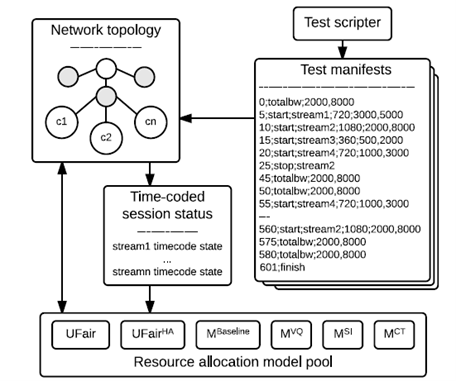
\includegraphics[scale=0.5]{images/topology.png}
\caption{Framework of evaluation testbed}
\label{fig:topology}
\end{figure}


\begin{figure}
\centering
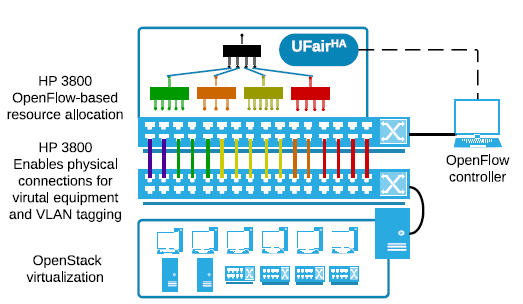
\includegraphics[scale=0.5]{images/switch.png}
\caption{OpenFlow-based experimentation}
\label{fig:switch}
\end{figure}


\section{Reading summary for \texorpdfstring{\cite{bhat_network_2017}}, by Jinwei}
In this paper, while the streaming clients retain full control of their existing adaptive streaming algorithms, the network assistance provided by the SABR architecture can significantly benefit both the streaming clients and the content providers in terms of QoE and content origin offloading. SABR utilizes information on available bandwidths per link and network cache contents to guide video streaming clients with the goal of improving the view's QoE. In addition, SABR uses SDN capabilities to dynamically program flows to optimize the utilization of CDN caches. 

One characteristic that distinguishes the widespread ABR video streaming systems from non-ABR systems is that for ABR, CDN caches may not contain all quality versions of a video. Thus, providing clients with information such as the presence of qualities of desired segments in particular caches allow the client to make an educated decision on segment retrieval. Additionally, providing bottleneck bandwidth information on the paths between the client and the caches that currently host the sought segments not only aids the client's decision but also eliminates the client's need to use less accurate bandwidth estimation methods such as end-to-end probing or application layer rate estimation. 

For the architecture design shown in Figure \ref{fig:sabr}, OpenFlow is used as the southbound API. The implementation is based on the work by Adrichem et al. \cite{openmon}. Since \cite{openmon} offers an accurate and precise OpenFlow Monitoring POX module. It monitors not only throughput, but also per flow packet loss and path delay for all flows and paths in use in an OpenFlow network. SABR also provides a northbound API for streaming clients to query available monitoring information, e.g. available bandwidth estimates and cache occupancy. Auto Regressive Integrated Moving Average(ARIMA) is used to predict the available bandwidth in the short term future. 

During SABR evaluation, an existing open source Python-based DASH client emulator is modified to implement the proposed SDN assisted adaption algorithm. Overall, each client makes the following requests: \textit{(i)} Initial HTTP GET request to the server or the nearest cache to retrieve Media Presentation Description (MPD) file for requested video; \textit{(ii)} HTTP GET request to SABR for a list of qualities of next segment(s) and the available bandwidth information to every advertised cache; \textit{(iii)} HTTP GET request to the selected cache to retrieve the desired segment.  

The performance evaluation metrics are partially based on metrics from \cite{zink05}. They include \textbf{Average Quality Bitrate, Number of Quality Switches, Spectrum, Rebuffering Ratio, Cache Hit Rate, Network Utilization, Server Load Ratio}. And the performance of SABR is compared with a set of different algorithms, like VLC, SQUAD and BOLA. 

\begin{figure}
\centering
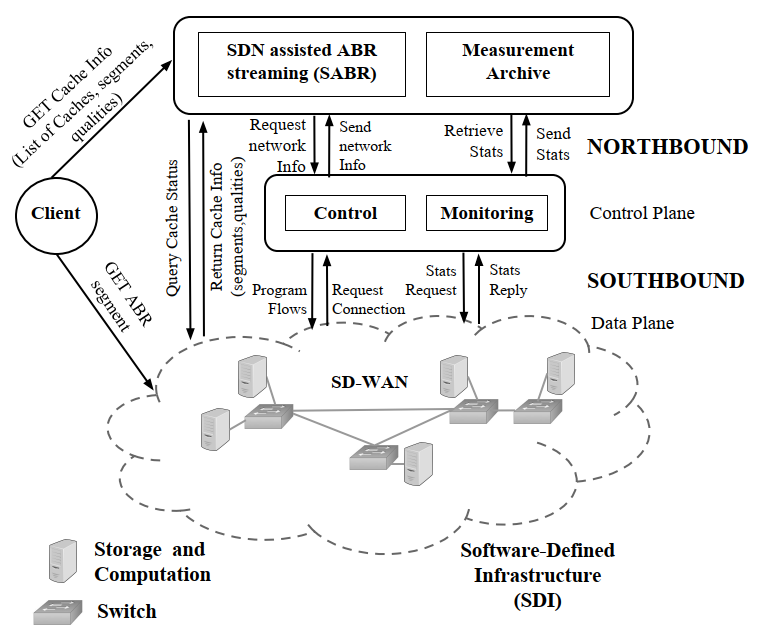
\includegraphics[scale=0.5]{images/sabr-arch.png}
\caption{SABR architecture design}
\label{fig:sabr}
\end{figure}

\section{Experience about CloudLab testbed}
During these two weeks, we created an account at the CloudLab testbed platform(\url{https://cloudlab.us/}). 

It seems that CloudLab is different from commercial cloud providers like AWS/Google Cloud in that each experiment(where VMs/bare metal nodes can be provisioned/allocated) has a default time limit of 16 hours. They will be terminated when they reach the time limit. Although the time limit for each experiment can be extended afterwards. You can also file a request to reserve nodes such that they would not expire during the time period you requested, e.g. 30 days. 

Since the resource of the testbed is limited, the original experiment topology mentioned in SABR\cite{bhat_network_2017} which requires more than 60 nodes might be difficult to allocate. We will modify the topology and reduce the nodes we need and use VMs instead of physical nodes in our experimental setup.

A screenshot of a bare metal server allocated on the CloudLab Utah cluster is shown in Figure \ref{fig:utah}. 

\begin{figure}
\centering
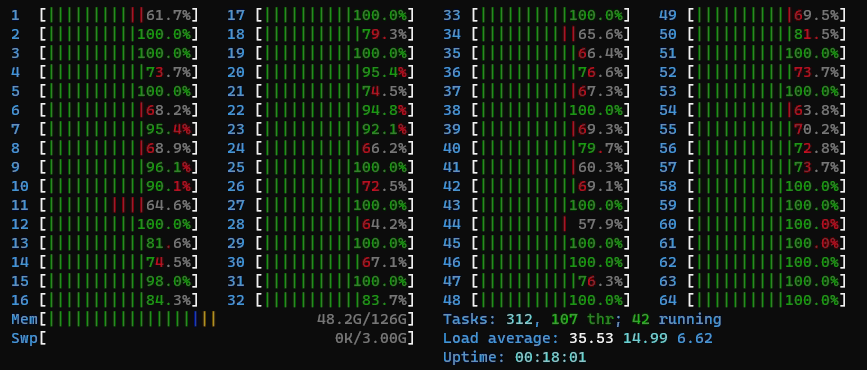
\includegraphics[width=\textwidth]{images/testbed.png}
\caption{Example of a bare metal server on CloudLab Utah cluster}
\label{fig:utah}
\end{figure}

Another screenshot of a XEN virtual machine allocated on the federated Emulab cluster is shown in Figure \ref{fig:vm}.

\begin{figure}
\centering
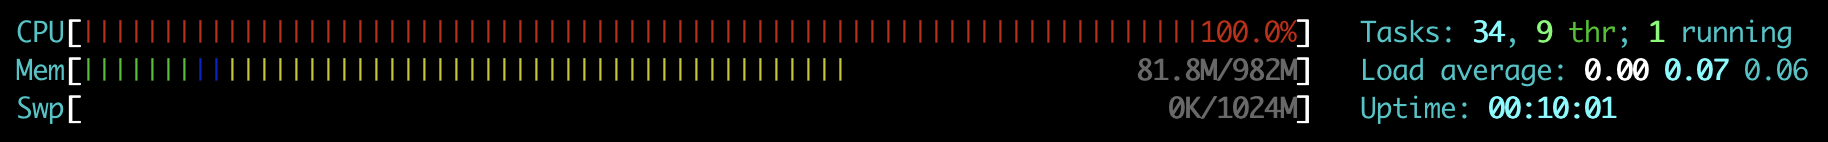
\includegraphics[width=\textwidth]{images/testbed vm.png}
\caption{Example of a XEN virtual machine on the federated Emulab cluster}
\label{fig:vm}
\end{figure}

\printbibliography

\end{document}